\documentclass[11pt]{article}
\usepackage[utf8]{inputenc}
\usepackage[czech]{babel}
%\usepackage[IL2]{fontenc}
\usepackage{times}
\usepackage[unicode]{hyperref}
\usepackage{multirow}
\usepackage[linesnumbered,ruled,noline,czech,longend]{algorithm2e}
\usepackage{graphics}
\usepackage{pdflscape}
\usepackage[a4paper, total={17cm, 24cm}, left=2cm, top=3cm]{geometry}

\urlstyle{same}

\begin{document}

\begin{titlepage}
\begin{center}
{\Huge \textsc{Vysoké učení technické v Brně}\\
\bigskip
{\huge \textsc{Fakulta informačních technologií}}} \\
\vspace{\stretch{0.382}}
{\LARGE Typografie a publikování\,--\,3. projekt}\\
\medskip
{\Huge Tabulky a obrázky} \\
\vspace{\stretch{0.618}}
\end{center}
{\Large \today \hfill Martin Zmitko (xzmitk01)}
\end{titlepage}

\section{Úvodní strana}
Název práce umístěte do zlatého řezu a nezapomeňte uvést dnešní datum a vaše jméno a příjmení.

\section{Tabulky}
Pro sázení tabulek můžeme použít buď prostředí \texttt{ tabbing } nebo prostředí \texttt{ tabular}.

\subsection{Prostředí \texttt{ tabbing}}
Při použití \texttt{ tabbing } vypadá tabulka následovně:
\begin{tabbing}
Vodní melouny \quad \= 27,40 \quad \= 2,5 kg \kill
\textbf{Ovoce} \> \textbf{Cena} \> \textbf{Množství}\\
Jablka \> 25,90 \> 3 kg\\
Hrušky \> 27,40 \> 2,5 kg\\
Vodní melouny \> 35,-- \> 1 kus
\end{tabbing}
\bigskip
Toto prostředí se dá také použít pro sázení algoritmů, ovšem vhodnější je použít 
prostředí \texttt{ algorithm } nebo \texttt{ algorithm2e } (viz sekce \ref{sec:3}).

\subsection{Prostředí \texttt{ tabular}}
Další možností, jak vytvořit tabulku, je použít prostředí \texttt{ tabular}. Tabulky pak 
budou vypadat takto\footnote{Kdyby byl problem s \texttt{ cline}, zkuste se podívat třeba sem: 
\url{http://www.abclinuxu.cz/tex/poradna/show/325037}}.
\bigskip

\begin{table}[h] 
    \catcode`\-=12
    \centering
    \begin{tabular}{|c|c|c|}
        \hline
        & \multicolumn{2}{c|}{\textbf{Cena}} \\ \cline{2-3}
        \textbf{Měna} & \textbf{nákup} & \textbf{prodej} \\ \hline
        EUR & 25,227 & 26,943 \\
        GBP & 29,368 & 31,492 \\
        USD & 21,260 & 22,661 \\ \hline
    \end{tabular}
    \caption{Tabulka kurzů k dnešnímu dni}
    \label{tab:1}
\end{table}

\bigskip

\begin{table}[h]
    \catcode`\-=12
    \centering
    \begin{tabular}{|c|c|} \hline
        $A$ & $\neg A$ \\ \hline
        \textbf{P} & N \\ \hline
        \textbf{O} & O \\ \hline
        \textbf{X} & X \\ \hline
        \textbf{N} & P \\ \hline
    \end{tabular}
    \begin{tabular}{|c|c|c|c|c|c|}
        \hline
        \multicolumn{2}{|c|}{\multirow{2}{*}{$A \wedge B$}} & \multicolumn{4}{c|}{$B$} \\ \cline{3-6} 
        \multicolumn{2}{|c|}{} & \textbf{P} & \textbf{O} & \textbf{X} & \textbf{N} \\ \hline
        \multirow{4}{*}{$A$} & \textbf{P} & P & O & X & N \\ \cline{2-6} 
        & \textbf{O} & O & O & N & N \\ \cline{2-6} 
        & \textbf{X} & X & N & X & N \\ \cline{2-6} 
        & \textbf{N} & N & N & N & N \\ \hline
    \end{tabular}
    \begin{tabular}{|c|c|c|c|c|c|}
        \hline
        \multicolumn{2}{|c|}{\multirow{2}{*}{$A \vee B$}} & \multicolumn{4}{c|}{$B$} \\ \cline{3-6} 
        \multicolumn{2}{|c|}{} & \textbf{P} & \textbf{O} & \textbf{X} & \textbf{N} \\ \hline
        \multirow{4}{*}{$A$} & \textbf{P} & P & P & P & P \\ \cline{2-6} 
        & \textbf{O} & P & O & P & O \\ \cline{2-6} 
        & \textbf{X} & P & P & X & X \\ \cline{2-6} 
        & \textbf{N} & P & O & X & N \\ \hline
    \end{tabular}
    \begin{tabular}{|c|c|c|c|c|c|}
        \hline
        \multicolumn{2}{|c|}{\multirow{2}{*}{$A \to B$}} & \multicolumn{4}{c|}{$B$} \\ \cline{3-6} 
        \multicolumn{2}{|c|}{} & \textbf{P} & \textbf{O} & \textbf{X} & \textbf{N} \\ \hline
        \multirow{4}{*}{$A$} & \textbf{P} & P & O & X & N \\ \cline{2-6} 
        & \textbf{O} & P & O & P & O \\ \cline{2-6} 
        & \textbf{X} & P & P & X & X \\ \cline{2-6} 
        & \textbf{N} & P & P & P & P \\ \hline
        \end{tabular}
    \caption{Protože Kleeneho trojhodnotová logika už je \uv{zastaralá}, uvádíme si zde příklad čtyřhodnotové logiky}
    \label{tab:2}
\end{table}

\section{Algoritmy} \label{sec:3}
Pokud budeme chtít vysázet algoritmus, můžeme použít prostředí \texttt{ algorithm}\footnote{Pro nápovědu, jak zacházet s prostředím \texttt{ algorithm}, můžeme zkusit tuhle stránku: \\
\url{http://ftp.cstug.cz/pub/tex/CTAN/macros/latex/contrib/algorithms/algorithms.pdf}} \quad nebo \texttt{  algorithm2e}\footnote{Pro \texttt{ algorithm2e } zase tuhle:
\url{http://ftp.cstug.cz/pub/tex/CTAN/macros/latex/contrib/algorithm2e/algorithm2e.pdf}.}. 
Příklad použití prostředí \texttt{ algorithm2e } viz Algoritmus \ref{alg:1}.
\bigskip

\begin{algorithm}
\label{alg:1}
\caption{\textsc{Fast}SLAM}
\SetNlSty{}{}{:}
\KwIn{$(X_{t - 1}, u_t, z_t)$}
\KwOut{$X_t$}
\BlankLine
\Indp\Indpp
\SetNlSkip{-1em}
$\overline{X_t} = X_t = 0$ \\
\For{$k = 1$ \emph{to} $M$}{
    $x_t^{[k]} =$ \emph{ sample\_motion\_model}$(u_t, x_{t - 1}^{[k]})$ \\
    $\omega_t^{[k]} =$ \emph{ measurement\_model}$(z_t, x_t^{[k]}, m_{t - 1})$ \\
    $m_t^{[k]} =$ \emph{ updated\_occupancy\_grid}$(z_t, x_t^{[k]}, m_{t - 1}^{[k]})$ \\
    $\overline{X_t} = \overline{X_t} + \langle x_x^{[m]}, \omega_t^{[m]} \rangle$
}
\For{$k = 1$ \emph{to} $M$}{
    draw \emph{i} wih probability $\approx \omega_t^{[i]}$ \\
    add $ \langle x_x^{[k]}, m_t^{[k]} \rangle$ to $X_t$
}
\Return{$X_t$}
\end{algorithm}

\section{Obrázky}
Do našich článků můžeme samozřejmě vkládat obrázky. 
Pokud je obrázkem fotografie, můžeme klidně použít bitmapový soubor. 
Pokud by to ale mělo být nějaké schéma nebo něco podobného, je dobrým zvykem takovýto obrázek vytvořit vektorově.

\begin{figure}[h]
    \centering
    \scalebox{0.4}{
        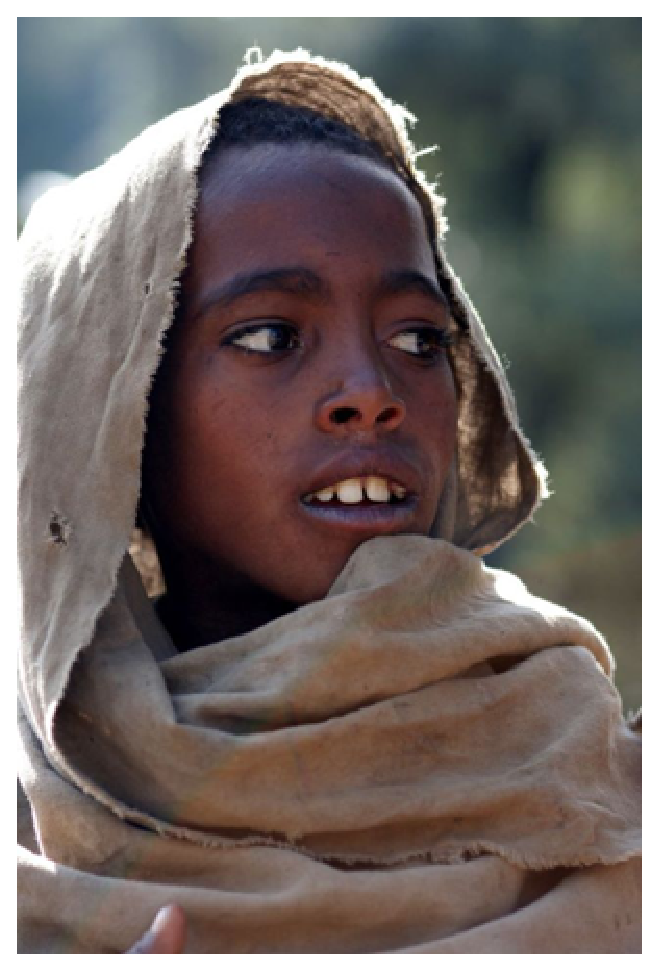
\includegraphics{etiopan.eps}
		\reflectbox{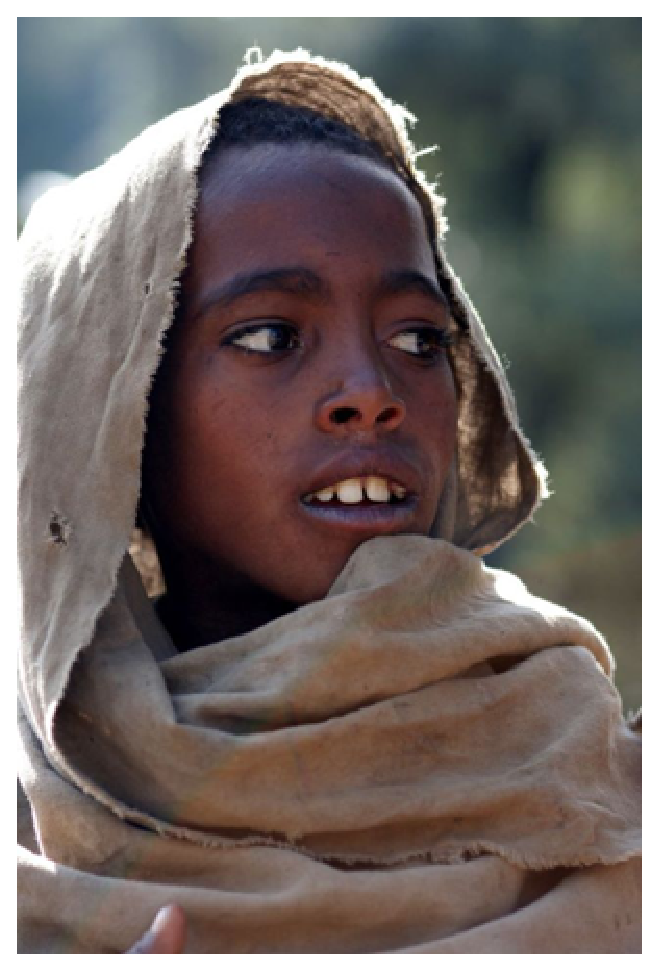
\includegraphics{etiopan.eps}}}
    \caption{Malý Etiopánek a jeho bratříček}
    \label{fig:1}
\end{figure}
\newpage

Rozdíl mezi vektorovým\,\dots
\begin{figure}[h]
    \centering
    \scalebox{0.4}{
\includegraphics{oniisan.eps}}
    \caption{Vektorový obrázek}
    \label{fig:2}
\end{figure}

\bigskip
\noindent \dots\,a bitmapovým obrázkem
\begin{figure}[h]
    \centering
    \scalebox{0.6}{
\includegraphics{oniisan2.eps}}
    \caption{Bitmapový obrázek}
    \label{fig:3}
\end{figure}
\bigskip

\noindent se projeví například při zvětšení.

Odkazy (nejen ty) na obrázky \ref{fig:1}, \ref{fig:2} a \ref{fig:3}, na tabulky \ref{tab:1} a \ref{tab:2} a také na algoritmus \ref{alg:1} jsou udělány pomocí křížových odkazů. 
Pak je ovšem potřeba zdrojový soubor přeložit dvakrát.

Vektorové obrázky lze vytvořit i přímo v \LaTeX u, například pomocí prostředí \texttt{ picture}.
\newpage

\begin{landscape}
\begin{figure}[h]
	\setlength{\unitlength}{1mm}
	\centering
	\begin{picture}(200, 110)
		\linethickness{1pt}
		\put(0, 0){\framebox(200, 100){}}
		\put(20, 80){\circle{14}}
		
		\linethickness{3pt}
		\put(141, 91){\circle{12}}
		\put(137, 91){\line(1,0){2}}
		
		\linethickness{1mm}
		\put(7, 15){\line(1, 0){184}}
        \put(31, 15){\line(0, 1){54}}
        \put(47, 89){\line(1, 0){87}}
        \put(159, 69){\line(0, -1){54}}
        \put(31, 69){\line(1, 0){56}}
        \put(89, 85){\line(1, 0){54}}
        \put(143, 85){\line(0, -1){70}}
        \put(89, 85){\line(0, -1){70}}
        
        \qbezier(31, 69)(39, 79)(47, 89)
        \qbezier(147, 87)(153, 78)(159, 69)
        
        \linethickness{0.5mm}
        \put(143, 85){\line(-1, 1){6}}
        \put(97, 79){\line(1, 0){38}}
        \put(135, 79){\line(0, -1){64}}
        \put(97, 79){\line(0, -1){64}}
        \put(143, 69){\line(1, 0){14}}
        \put(117, 79){\line(0, -1){22}}
        \put(117, 57){\line(1, 0){18}}
        \put(109, 57){\line(-1, 0){12}}
        \put(109, 57){\line(0, 1){22}}
        \put(117, 39){\line(0, -1){24}}
        \put(109, 39){\line(-1, 0){12}}
        \put(109, 39){\line(0, -1){24}}
        \put(117, 39){\line(1, 0){18}}
        \put(71, 39){\line(0, -1){24}}
        \put(71, 39){\line(-1, 0){30}}
        \put(41, 39){\line(0, -1){24}}
        \put(51, 39){\line(0, -1){24}}
        \put(53, 85){\line(-1, -3){4}}
        \put(49, 73){\line(1, 0){8}}
        \put(57, 73){\line(1, 3){4}}
        \put(61, 85){\line(-1, 0){8}}
        
        \linethickness{0.25mm}
        \put(117, 77){\line(1, 0){18}}
        \put(117, 75){\line(1, 0){18}}
        \put(117, 73){\line(1, 0){18}}
        \put(117, 71){\line(1, 0){18}}
        \put(117, 69){\line(1, 0){18}}
        \put(117, 67){\line(1, 0){18}}
        \put(117, 65){\line(1, 0){18}}
        \put(117, 63){\line(1, 0){18}}
        \put(97, 77){\line(1, 0){12}}
        \put(97, 75){\line(1, 0){12}}
        \put(97, 73){\line(1, 0){12}}
        \put(51, 37){\line(1, 0){20}}
        \put(51, 35){\line(1, 0){20}}
        \put(51, 33){\line(1, 0){20}}
        \put(51, 31){\line(1, 0){20}}
        
	\end{picture}
	\caption{Vektorový obrázek mého bydlení}
\end{figure}
\end{landscape}
\end{document}
